\documentclass[aspectratio=169]{beamer}
%Information
\title{Hecke L-函数的解析延拓}
\titlegraphic{\hfill
\includegraphics[height=1cm]{xjtu.png}}
% \institute{西安交通大学}
\author{王尔卓 \, \newline 指导老师: 郭振宇}

% \date{July 6,2024}
%Theme
\usetheme[block=fill, sectionpage=none]{metropolis}
\useoutertheme{infolines}
\useinnertheme{metropolis}
\setbeamertemplate{blocks}[rounded][shadow=false]
\setbeamertemplate{items}[ball]
\setbeamertemplate{sections/subsections in toc}[ball]
\setbeamertemplate{headline}{}
\usecolortheme{custom}
%\usetheme{Madrid}
%\usetheme{Heverlee}

%Setting
\usepackage[UTF8,noindent]{ctexcap}
\theoremstyle{definition}
\newtheorem{defn}{Definition}[section]
\newtheorem{coro}[defn]{Corollary}
\newtheorem{theo}[defn]{Theorem}
\newtheorem{exer}[defn]{Exercise}
\newtheorem{rema}[defn]{Remark}
\newtheorem{lem}[defn]{Lemma}
\newtheorem{prop}[defn]{Proposition}
\newtheorem{nota}[defn]{Notation}
\newtheorem{exam}[defn]{Example}

\newenvironment{prooff}{{\noindent\it\textcolor{cyan!40!black}{Proof}:}\,}{\par}
\newenvironment{proofff}{{\noindent\it\textcolor{cyan!40!black}{Proof of the lemma}:}\,}{\qed \par}
\newcommand{\bbrace}[1]{\left\{ #1 \right\} }
\newcommand{\bb}[1]{\mathbb{#1}}
\newcommand{\p}{^{\prime}}
\renewcommand{\mod}[1]{(\text{mod}\,#1)}
\newcommand{\blue}[1]{\textcolor{blue}{#1}}
\newcommand{\spec}[1]{\text{Spec}({#1})}
\newcommand{\rarr}[1]{\xrightarrow{#1}}
\newcommand{\larr}[1]{\xleftarrow{#1}}
\newcommand{\emptyy}{\underline{\quad}}
\newenvironment{enu}{\begin{enumerate}[(1)]}{\end{enumerate}}
%ctrl+点击文本返回代码  选中代码 ctrl+alt+j 为代码查找文本

\begin{document}
\begin{frame}
    \titlepage
\end{frame}
\begin{frame}{Riemann zeta 函数 与 Dirchlet L-函数}
    Riemann zeta 函数$\zeta(s)$ 和Dirchlet L-函数$L(s,\chi)$ 是数论中两个非常重要的研究对象. 
    $\zeta(s)$ 的定义为
    \begin{equation*}
        \zeta(s)=\sum_{n=1}^{\infty}\frac{1}{n^s}, \quad \text{Re}(s)>1.  
    \end{equation*}
 
\end{frame}
\begin{frame}{Riemann zeta 函数 与 Dirchlet L-函数} 
    通过Possion Summation Formula 我们可以得到$\zeta(s)$的解析延拓和函数方程.
    定义$\xi(s)=\pi^{-s/2}\Gamma(s/2)\zeta(s)$, 可以证明$\xi(s)$可以亚纯延拓到整个
    复平面并满足: 
    \begin{equation*}
        \xi(s)=\xi(1-s), s\in\bb{C}-\bbrace{0,1}
    \end{equation*}
通过延拓后的Riemann zeta 函数$\zeta(s)$的解析性质以及复变函数的工具,  
最终可以证明素数定理
\begin{equation*}
    \pi(x)\sim \text{Li}(x).
\end{equation*}

\end{frame}
\begin{frame}{Riemann zeta 函数 与 Dirchlet L-函数}
    一个模$m$ Dirchlet特征是指一个群同态 $(\bb{Z}/m\bb{Z})^\times \rightarrow \bb{C}^\times$, 
    我们可以定义Dirchlet L-函数 
    \begin{equation*}
        L(s,\chi)=\sum_{(n,m)=1}\frac{\chi(n)}{n^s}, \quad \text{Re}(s)>1.  
    \end{equation*} 
    与$\zeta(s)$类似的是, Dirchlet L-函数也有解析延拓与函数方程.
    
    设 $\chi$ 为模 $N$ 的本原特征. 令
    % $$
    % \begin{gathered}
    % \delta(\chi)=\delta=\left\{\begin{array}{l}
    % 0, \text { 若 } \chi(-1)=1 ; \\
    % 1, \text { 若 } \chi(-1)=-1,
    % \end{array}\right. \\
    % \xi(s, \chi)=\left(\frac{N}{\pi}\right)^{s / 2} \Gamma\left(\frac{s+\delta}{2}\right) L(s, \chi),
    % \end{gathered}
    % $$ 
    \begin{equation*}
        \xi(s, \chi)=\left(\frac{N}{\pi}\right)^{s / 2} \Gamma\left(\frac{s+\delta}{2}\right) L(s, \chi)
    \end{equation*}
        则 $L(s, \chi)$ 可以解析延拓到整个复平面上并且满足如下的函数方程 
        $$
        \xi(s, \chi)=\frac{G(1, \chi)}{i^\delta \sqrt{N}} \xi(1-s, \bar{\chi}) .
        $$
\end{frame}
\begin{frame}{推广L函数的定义}
    随着研究的深入, 一些数学工作者的兴趣从$\bb{Q}$本身拓展为为更一般的代数数域, 也就是$\bb{Q}$的有限次扩张. 
    而对于一般的代数数域的研究, 原有的Riemann zeta函数$\zeta(s)$
    以及Dirchlet L-函数这些工具显得有些力不从心.
    这时我们需要推广zeta函数和L函数的定义, 使得其成为
    更一般的, 能刻画一个代数数域性质的L函数. 

    从历史上来看, L-函数的推广分为两个支流.
    第一侧是所谓“伽罗瓦侧”的Artin L-函数, 另一侧是自守侧的Hecke L-函数. 
    
\end{frame}

\begin{frame}{第一种方式: Artin L-函数}
考虑一个代数数域的伽罗瓦扩张
$L/K$, 记伽罗瓦群为$\text{Gal}(L/K)$. 考虑一个$\mathcal{O}_L$中的素理想$\mathfrak{P}$, 
其分解群, 惯性群, 分解域, 惯性域按如下对应排开: 
\begin{figure}
    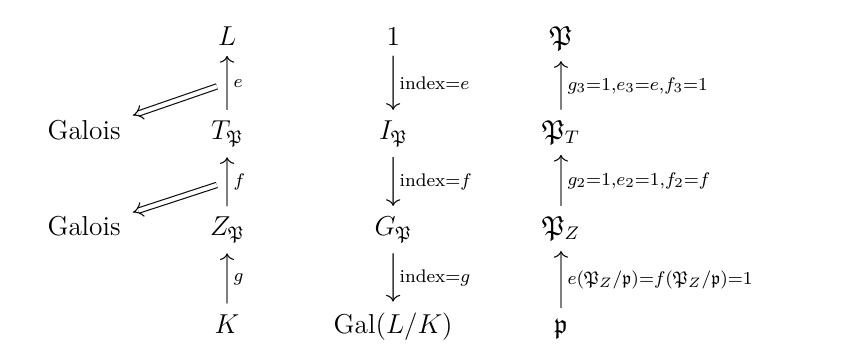
\includegraphics[height=0.5\textheight]{artin-L.png}
\end{figure}

\end{frame}
\begin{frame}{第一种方式: Artin L-函数}
    并且有典范同构
    $$
    G_{\mathfrak{P}} / I_{\mathfrak{P}}\simeq \text{Gal}(\kappa(\mathfrak{P})/\kappa(\mathfrak{p}))
    $$
    因此, $G_{\mathfrak{P}} / I_{\mathfrak{P}}$ 由所谓的Frobenius Automorphism 
    $\varphi_{\mathfrak{P}}$生成.
    其在$\text{Gal}(\kappa(\mathfrak{P})/\kappa(\mathfrak{p}))$的像为
    $x \mapsto x^q$, 其中$q=|\kappa(\mathfrak{p})|$.注意到因为我们没有假设
    $\mathfrak{p}$非分歧, 此时Frobenius Automorphism 依赖于代表元的选取. 
    
    考虑伽罗瓦群的一个有限维复表示
    $\rho: \text{Gal}(L/K)\rightarrow \text{GL}(V)$, 注意到Frobenius Automorphism 
    $\varphi_{\mathfrak{P}}$ 以及这个伽罗瓦群的表示自然诱导出一个$V^{I_\mathfrak{P}}$($I_\mathfrak{P}$作用下的不变子空间)
    上的有限阶可逆线性映射. 具体定义为
    \begin{equation*}
        \varphi_{\mathfrak{P}}: V^{I_\mathfrak{P}}\rightarrow V^{I_\mathfrak{P}}, v\mapsto \rho(\varphi_{\mathfrak{P}})v 
    \end{equation*} 
\end{frame}
\begin{frame}{第一种方式: Artin L-函数}
    注意到这个线性映射的特征多项式
    $$
        \operatorname{det}\left(1-\varphi_{\mathfrak{P}}t; V^{I_{\mathfrak{P}}}\right)\in \bb{C}[t]
    $$   
    并不依赖于$\mathfrak{P}$以及代表元的选取, 且可以展开成
    \begin{equation}
        \operatorname{det}\left(1-\varphi_{\mathfrak{P}}t ; V^{I_{\mathfrak{P}}}\right)=\prod_{i=1}^d\left(1-\varepsilon_i t\right)
        \label{equation: characteristic polynomial, Frobenious Automorphism}
    \end{equation}
    其中 $\varepsilon_i$ 为一些单位根.
    因此我们定义一个伽罗瓦群表示$\rho$的Artin L-函数为 
    $$
    \mathcal{L}(L/K, \rho, s)=\prod_{\mathfrak{p}} \frac{1}{\operatorname{det}(1-\varphi_{\mathfrak{P}}
    \mathfrak{N}(\mathfrak{p})^{-s} ; V^{I_{\mathfrak{P}}}) },\text{Re}(s)>1
    $$
    从(\ref{equation: characteristic polynomial, Frobenious Automorphism})式
    可以看出上式在实部大于$1$里内闭一致收敛
    且全纯. 
\end{frame}


\begin{frame}{Restricted Direct Product}
    \begin{defn}[Restricted Direct Product]
        对指标集 $J=\{\nu\}$ 每个元素给一个LCHG(locally compact Hausdorff topological group) 
        $G_\nu$.
        $J_{\infty}$ 是一个$J=\{\nu\}$的有限子集. 
        对每个 $\nu \notin J_{\infty}$, 给一个紧开子群
        $H_\nu \leq G_\nu$. 
        则$G_v$关于紧开子群$H_\nu$的
        restricted direct product定义为
        $$
        G=\prod_{\nu \in J}^{\prime} G_\nu=\left\{\left(x_\nu\right): x_\nu \in G_\nu, x_\nu \in H_\nu \text { 除了有限个 } \nu\right\}
        $$
    \end{defn}
    \begin{exam}[adèle and idèle]
        $\mathbb{A}_K$:考虑代数数域$K$每个prime divisor处的完备化$K_\nu$, 对finite place 定义紧开子群$\mathcal{O}_\nu$, 则 
        $\mathbb{A}_K$为这些$K_\nu$的restricted direct product. 

        $\mathbb{I}_K$:考虑代数数域$K$每个prime divisor处的完备化$K_\nu$, 对finite place 的$K_\nu^\times$
        定义紧开子群$\mathcal{O}_\nu^\times$, 则 
        $\mathbb{I}_K$为这些$K_\nu^\times$的restricted direct product. 
    \end{exam}
\end{frame}
\begin{frame}{Characters of Restricted Direct Product of LCHA}
    令 $G$ 是restricted direct product of $G_\nu$. 
    作为拓扑群, 我们有同构
    $$
    \hat{G} \cong \prod^{\prime} \hat{G}_\nu
    $$
    其中右侧Restricted Direct Product中每个拓扑群分量的紧开子群取为
    $$
    K\left(G_\nu, H_\nu\right)=\left\{\chi_\nu \in \hat{G}_\nu:\left.\chi_\nu\right|_{H_\nu}=1\right\}
    $$
    对所有 $\nu \notin J_{\infty}$. 
\end{frame}
\begin{frame}{局部域乘法群的特征}
    局部域是指$\bb{R},\bb{C},$ $\bb{Q}_p$的有限次扩张, 则
    \begin{enu}
        \item $F=\mathbb{R}$时, $\mathbb{R}^\times$的quasi-character 形如$|\cdot|^s$ or $\text{sgn}|\cdot|^s $.
        \item $F=\mathbb{C}$时, 
        $\mathbb{C}^\times$的quasi-character形如
        $$
        \chi_{s, n}: r e^{i \theta} \mapsto r^s e^{i n \theta},s\in\bb{C}, n\in\bb{Z}
        $$
        \item 如果$F$non-Archimedean, 令$\mathfrak{p}$ 
        为$F$赋值环的唯一极大理想.
        则存在非负整数$n \in \mathbb{N}$ 使得$\chi_0\left(1+\mathfrak{p}^n\right)=\{1\}$. 取最小这样的$n$, 
        我们称$\mathfrak{p}^n$ 为 $\chi_0$的conductor. 
        如果我们固定$\pi_F$为一个$\mathfrak{p}$的生成元, 
        我们可以找到唯一$\chi_0$满足$\chi(\pi_F)=1$
        和唯一$s\in \bb{C}/\dfrac{2\pi i}{\log q}\bb{Z}$ 使得 $\chi=\chi_0|\cdot|^s$.
    \end{enu}
\end{frame}
\begin{frame}{第二种方式: Hecke L-函数}

    Local L-函数: 令 $\chi \in \operatorname{Hom}_{\text {cont }}\left(F^{\times}, \mathbb{C}^{\times}\right)$.
    \begin{enu} 
        \item 如果 $F=\mathbb{C}$, 令
        $$
        L\left(\chi_{s, n}\right)=\Gamma_{\mathbb{C}}\left(s+\frac{|n|}{2}\right)=(2 \pi)^{-\left(s+\frac{|n|}{2}\right)} \Gamma\left(s+\frac{|n|}{2}\right)
        $$
        \item 如果 $F=\mathbb{R}$ 且 $\chi=|\cdot|^s$ 或者 $\chi=\text{sgn}|\cdot|^s$, 令
        $$
        L(\chi)= \begin{cases}\Gamma_{\mathbb{R}}(s)=\pi^{-s / 2} \Gamma(s / 2) & \text { 如果} \chi=|\cdot|^s \\ \Gamma_{\mathbb{R}}(s+1) & \text { 如果} \chi=\text{sgn}|\cdot|^s\end{cases}
        $$
        \item 如果 $F$ is non-Archimedean, 令
        $$
        L(\chi)= \begin{cases}\left(1-\chi\left(\pi_F\right)\right)^{-1} & \text { 如果} \chi \text { unramified } \\ 1 & \text { otherwise }\end{cases}
        $$
    \end{enu}
   

\end{frame}
\begin{frame}{第二种方式: Hecke L-函数}
    \begin{defn}
        定义
        $$
        L(\chi)=\prod_\nu L\left(\chi_\nu\right)
        $$
        注意到 $L(\chi)$ 在 $\text{Re}(s)>1$的紧子集上一致收敛且在$\text{Re}(s)>1$上全纯.
    \end{defn}
    \begin{defn}[Hecke L-function]
        令 $\chi \in \operatorname{Hom}_{\text {cont }}\left(\mathbb{I}_K / K^*, \mathbb{C}^{\times}\right)$是一个unitary idele-class character. 
        对复数$s$, 定义Hecke L-函数$L(s, \chi)$为
        $$
        L(s, \chi)=L\left(\chi|\cdot|^s\right), \text{Re}(s)>1
        $$
    \end{defn}
\end{frame}


\begin{frame}{函数方程}
    现在一个很容易想到的问题是就是, 我们所给出的两种推广的L-函数
    Artin L-函数和Hecke L-函数
    是否也有与Riemann zeta函数, Dirchlet L-函数类似的解析延拓和函数方程呢? 
    这个问题是我毕业论文的主题.  

    接下来我们要说明的是, 本质上\blue{Artin L-函数 函数方程的建立}可以转化为
    \blue{Hecke L-函数函数方程的建立}, 因此只用考虑Hecke 
    L-函数的情况. 
\end{frame}




\begin{frame}{Artin L-函数的性质}
   
        $L/K$ 是一个Galois扩张, $G=\text{Gal}(L/K)$.
    \begin{enu}   
        \item (additive) 如果 $\rho,\rho\p$是两个$G$的复表示, 则
        $$
        \mathcal{L}\left(L/K, \rho\oplus \rho\p, s\right)=\mathcal{L}(L/K, \rho\p, s) \mathcal{L}\left(L/K, \chi^{\prime}, s\right)
        $$
        \item (invariant under projection) 考虑一个更大的Galois扩张
        $L^{\prime}/K, L^{\prime} \supseteq L \supseteq K$.
        $\rho$是$\text{Gal}(L/K)$的一个表示.
        注意到 $G\rarr{\pi} G/\text{Gal}(L/M)\simeq \text{Gal}(L/K)$,
        $\rho\circ \pi$ 为 $G$的一个表示.
        我们有
        $$
        \mathcal{L}\left(L^{\prime}/K, \rho\circ \pi, s\right)=\mathcal{L}(L/K, \rho, s) .
        $$
        \item (invariant under inflation) 如果 $M$是一个中间域, $L \supseteq M \supseteq K$, 
        且$(\rho,V)$ 是$H=\text{Gal}(L/M)$的一个的表示, 
        则
        $$
        \mathcal{L}(L/M, \rho, s)=\mathcal{L}\left(L/K, \text{Ind}_{H}^G(\rho), s\right) .
        $$
    \end{enu}
    
\end{frame}
\begin{frame}{Artin L-函数的函数方程}
    下面我们简要说明Artin L-函数的函数方程构建思路, 首先根据任意伽罗瓦群的表示可以由
    Brauer定理写成一些子群的1维表示的诱导表示的整系数和. 根据性质(1)和(3), 只需要对1维表示
    证明函数方程. 由于这些子群可能非Abel, 但注意到一个群的1维表示一定factor through这个群的交换化, 
    因此由性质(2)只需证明Abel群1维表示的函数方程. 由Artin互反律, 这等价于构建Hecke L-函数的函数方程. 
\end{frame}




\begin{frame}{课题执行方案}
    目前已经通过Tate的原文以及其他数学工作者的笔记了解了原文的脉络和技术, 后续主要
    阅读一些与Tate's thesis相关的应用, 
    以及尽可能了解高维情况的自守形式 L-函数.
    \begin{enu}
        \item 12月-2月: 完成文献翻译, 完整阅读Artin L-函数函数方程的建立, 初步整理Tate's thesis的证明.
        \item 2月-5月 : 完善Tate's thesis的证明梳理, 
        阅读Bump的自守形式与自守表示以及其他材料了解高维情况的结果并将部分内容整理至毕业论文中.
    \end{enu}
\end{frame}



\end{document}